% !TeX root = er.tex

\chapter{Controle de Lógica Fuzzy}\label{ch.fuzzy}

Os algoritmos de controle do capítulo~\ref{ch.control} usaram cálculos matemáticos exatos para determinar os sinais usados para controlar o comportamento de um robô. Uma abordagem alternativa é usar algoritmos de controle \emph{fuzzy logic} baseados em \emph{rules}. Um sistema de controle de cruzeiro pode ter regras da forma:
\begin{itemize}
\item Se o \emph{carro na frente está longe} ou o \emph{carro atrás está perto}, definir a \emph{velocidade para o jejum}.
\item Se o carro da frente estiver próximo, defina a velocidade para diminuir.
\end{itemize}
A lógica é ``fuzzy'' porque as regras são expressas em termos de \emph{variáveis lingüísticas} como \emph{velocidade} cujos valores não têm definições matemáticas precisas, mas apenas especificações lingüísticas imprecisas como \emph{fast} e \emph{slow}.

Um controlador de lógica difusa consiste em três fases que são executadas sequencialmente:

\begin{description}
\item[\textbf{Fuzzify}] Os valores dos sensores são convertidos em valores das variáveis lingüísticas, tais como: \p{far}, \p{fechar}, \p{near}, chamadas \emph{premises}. Cada premissa especifica uma \emph{certeza} que é a probabilidade de nossa crença de que a variável é verdadeira.
\item[\textbf{Aplicar regras}] Um conjunto de \emph{rules} expressa o algoritmo de controle. Dado um conjunto de premissas, infere-se um \emph{consequente}. As conseqüências também são variáveis lingüísticas, tais como: \p{muito rápido}, p{rápido}, \p{lento}, \p{baixo}, \p{parado}.
\item[\textbf{Defuzzify}] As conseqüências são combinadas para produzir uma saída \emph{crisp}, que é um valor numérico que controla algum aspecto do robô, como a potência aplicada aos motores.
\end{description}

As seções seguintes apresentam as três fases do controle difuso para a tarefa de um robô se aproximar de um objeto e parar quando ele está muito próximo do objeto.

\section{Fuzzify}

Ao se aproximar de um objeto, o valor lido pelo sensor de proximidade horizontal aumenta de $0$ para $100$. O valor retornado pelo sensor é fuzzificado convertendo-o para um valor de uma variável lingüística. A Figura~\ref{fig.fuzz} mostra três gráficos para converter os valores do sensor em certezas das variáveis lingüísticas \p{far}, \p{fechar} e \p{near}. O eixo $x$ é o valor retornado pelo sensor e o eixo $y$ dá a premissa para cada variável, a certeza de que a variável lingüística é verdadeira.

\begin{figure}
\begin{center}
% Fuzzify a horizontal proximity sensor
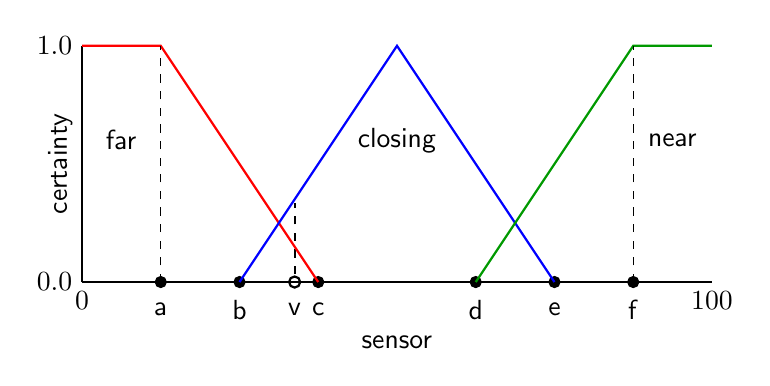
\begin{tikzpicture}
\draw (0,0) node[left] {\p{0.0}} node[below] {\p{0}} -- node[sloped,above] {\textsf{certainty}} (0,3) node[left] {\p{1.0}};
\draw (0,0) -- node[below,yshift=-16pt] {\textsf{sensor}} (8,0) node[below] {\p{100}};
\foreach \n/\x in {a/1,b/2,c/3,d/5,e/6,f/7} {
  \draw[fill] (\x,0) circle [radius=2pt];
  \node at (\x,-10pt) { \textsf{\n} };
}
\draw[thick] (2.7,0) circle [radius=2pt];
\node at (2.7,-10pt) { \textsf{v} };
\draw[dashed,thick] (2.7,.1) -- +(0,.9);
\draw[red,thick] (0,3) -- (1,3) -- (3,0);
\draw[blue,thick] (2,0) -- (4,3) -- (6,0);
\draw[green!60!black,thick] (5,0) -- (7,3) -- (8,3);
\draw[dashed] (1,0) -- (1,3);
\draw[dashed] (7,0) -- (7,3);
\node at (.5,1.8) {\textsf{far}};
\node at (4,1.8) {\textsf{closing}};
\node at (7.5,1.8) {\textsf{near}};
\end{tikzpicture}
\caption{Fuzzify o valor do sensor de proximidade horizontal}\label{fig.fuzz}
\end{center}
\end{figure}

Os pontos etiquetados no eixo $x$ referem-se a limites: (a) \p{muito baixo}, (b) \p{fechamento baixo}, (c) \p{muito alto}, (d) \p{quase baixo}, (e) \p{fechamento alto}, (f) \p{quase alto}. Se o valor do sensor estiver abaixo \p{muito baixo}, então estamos completamente certos de que o objeto está longe e a certeza é de $1$. Se o valor estiver entre \p{fechamento baixo} e \p{muito alto} então temos alguma certeza de que o objeto está longe, mas também alguma certeza de que ele está fechando. A confusão resulta da sobreposição de faixas: quando o valor está entre o ponto (b) e o ponto (c), não podemos dizer com total certeza se o objeto está longe ou se está fechando. Para o valor do sensor \p{v} de cerca de $33$, a certeza de \p{far} é de cerca de $,15$ e a certeza de \p{fechamento} é de cerca de $,25$.

\section{Aplicar regras}

As três premissas, as certezas de \p{longe}, \p{fechar} e \p{perto de}, são usadas para calcular cinco conseqüências usando as seguintes regras:

\begin{enumerate}
\item Se \p{longe} então \p{muito rápido}
\item Se \p{longe} e \p{fechamento} então \p{rápido}
\item Se \p{fechamento} então \p{cruzeiro}
\item Se \p{fechamento} e \p{perto de} então \p{lento}
\item Se \p{perto de} então \p{parar}
\end{enumerate}

As certezas das conseqüências resultantes das regras 1, 3, 5 são as mesmas que as certezas das premissas correspondentes. Quando há duas premissas, como nas regras 2 e 4, as certezas das conseqüências são calculadas a partir do mínimo das certezas das premissas. Uma vez que \emph{ambas} as premissas devem ser aplicadas, não podemos ter \emph{mais certeza} das conseqüências do que da menor das premissas. Para o valor \p{v} na Fig.~\ref{fig.fuzz}, aplica-se a regra 2 e a certeza do conseqüente é $\min(.15,.25)=.15$.

Another way of combining premises is to take their joint probability:
\[
p(A \cap B) = P(A)\cdot P(B)\,.
\]
Para o valor \p{v}, a certeza do conseqüente é de $,15\times .25= .0375$, muito menos do que a certeza obtida a partir da função mínima.

\section{Defuzzify}

O próximo passo é combinar as conseqüências, levando em conta suas certezas. A figura~\ref{fig.defuzz} mostra as potências do motor de saída para cada uma das cinco conseqüências. Por exemplo, se estivermos completamente certos de que a saída é \emph{cruise}, o gráfico central na figura mostra que a potência do motor deve ser ajustada para $50$, mas se estivéssemos menos certos, a potência do motor deve ser menor ou maior.

\begin{figure}
\begin{center}
% Defuzzify to obtain a crisp motor setting
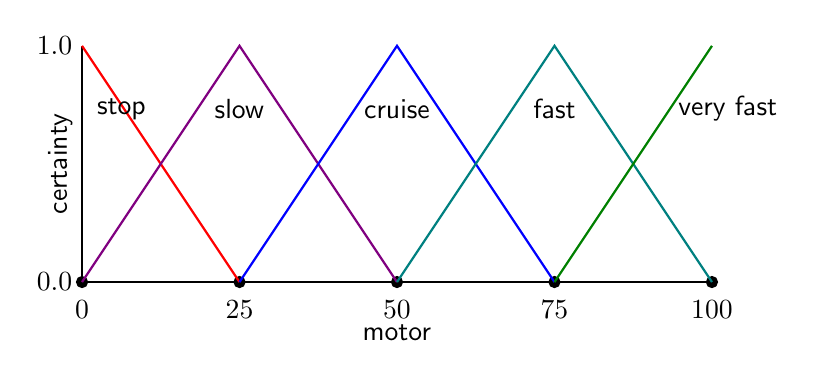
\begin{tikzpicture}
\draw (0,0) node[left] {\p{0.0}} -- node[sloped,above] {\textsf{certainty}} (0,3) node[left] {\p{1.0}};
\draw (0,0) -- node[below,yshift=-12pt] {\textsf{motor}} (8,0);
\foreach \n/\x in {0/0,25/2,50/4,75/6,100/8} {
  \draw[fill] (\x,0) circle [radius=2pt];
  \node at (\x,-10pt) { \p{\n} };
}
\draw[red,thick] (0,3) -- (2,0);
\draw[red!50!blue,thick] (0,0) -- (2,3) -- (4,0);
\draw[blue,thick] (2,0) -- (4,3) -- (6,0);
\draw[blue!50!green,thick] (4,0) -- (6,3) -- (8,0);
\draw[green!50!black,thick] (6,0) -- (8,3);
\node at (.5,2.2) {\textsf{stop}};
\node at (2,2.2) {\textsf{slow}};
\node at (4,2.2) {\textsf{cruise}};
\node at (6,2.2) {\textsf{fast}};
\node at (8.2,2.2) {\textsf{very fast}};
\end{tikzpicture}
\caption{Desfuzzify para obter o ajuste do motor crocante}\label{fig.defuzz}
\end{center}
\end{figure}

Suponha que a certeza da conseqüência do \emph{cruise} seja computada como sendo de $0,4$. Então o triângulo central na Fig.~\ref{fig.defuzz} não é mais relevante porque a certeza nunca pode ser maior que $0,4$, que é exibido como um trapézio na Fig.~\ref{fig.trap}.

\begin{figure}
\begin{center}
% Areas defined by the certainties of the consequents
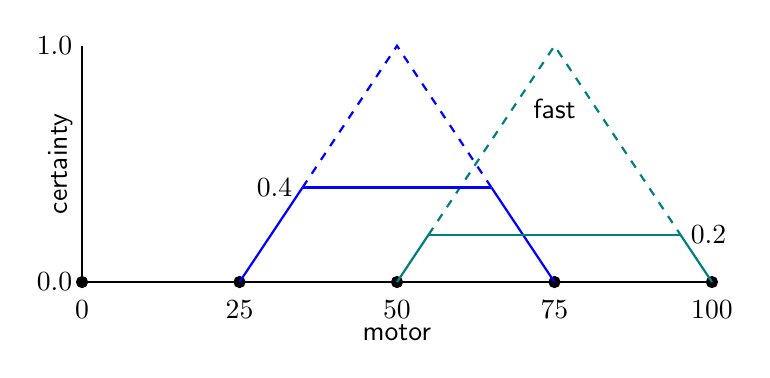
\begin{tikzpicture}
\draw (0,0) node[left] {\p{0.0}} -- node[sloped,above] {\textsf{certainty}} (0,3) node[left] {\p{1.0}};
\draw (0,0) -- node[below,yshift=-12pt] {\textsf{motor}} (8,0);
\foreach \n/\x in {0/0,25/2,50/4,75/6,100/8} {
  \draw[fill] (\x,0) circle [radius=2pt];
  \node at (\x,-10pt) { \p{\n} };
}
\draw[blue,thick] (2,0) -- (2.8,1.2);
\draw[blue,thick] (5.2,1.2) -- (6,0);
\draw[blue,thick,dashed] (2.8,1.2) -- (4,3) -- (5.2,1.2);
\draw[blue!50!green,thick] (4,0) -- (4.4,.6);
\draw[blue!50!green,thick] (7.6,.6) -- (8,0);
\draw[blue!50!green,thick,dashed] (4.4,.6) -- (6,3) -- (7.6,.6);
node at (4,2.2) {\textsf{cruise}};
\node at (6,2.2) {\textsf{fast}};
\draw[blue,thick] (2.8,1.2) node[black,left] {\p{0.4}} -- (5.2,1.2);
\draw[blue!50!green,thick] (4.4,.6) -- (7.6,.6) node[black,right] {\p{0.2}};
\end{tikzpicture}
\caption{Áreas definidas pelas certezas das conseqüências}\label{fig.trap}
\end{center}
\end{figure}

Que $w$ e $h$ sejam a largura e a altura de um triângulo. Então a área de um trapézio delimitada pela linha à altura $h'$ é dada pela fórmula:\footnote{A derivação da fórmula é dada no Apêndice~\ref{a.trap}.}
\begin{displaymath}
wh'\left(1-\frac{h'}{2h}\right)\,.
\end{displaymath}
É possível que mais de uma conseqüência tenha valores positivos. A figura~\ref{fig.trap} mostra os trapézios para o conseqüente \p{cruzeiro} com uma certeza de $0,4$ e o conseqüente \p{rápido} com uma certeza de $0,2$. Para $w=50$, $h=1$, $h_{c}'=0,4$ (\p{cruzeiro}), $h_{f}'=0,2$ (\p{rápido}), as áreas dos trapézios $a_c$ (\p{cruise}) e $a_f$ (\p{rápido}) são:
\begin{displaymath}
\spacearray
\begin{array}{l}
a_c = 50\times 0.4 \left(1 - \frac{0.4}{2}\right) = 16\\
a_f = 50\times 0.2 \left(1 - \frac{0.2}{2}\right) = 9\,.
\end{array}
\end{displaymath}
Para obter um valor nítido, o \emph{centro de gravidade} é computado. Esta é a soma das áreas dos trapézios ponderadas pelo valor no centro da base de cada trapézio dividido pela soma das áreas:
\begin{displaymath}
\frac{16\times 50 + 9\times 75}{16+9}=59\,.
\end{displaymath}
Tvalor está mais próximo do valor associado com o \p{cruzeiro} do que do valor associado com o \p{rápido}. Isto não é surpreendente, já que a certeza de que a \p{cruzeiro} é maior do que a certeza de que o café da manhã é \p{rápido}.

\begin{framed}
\act{Lógica fuzzy}{fuzzy}
\begin{itemize}
\item Implementar o controlador de lógica difusa para um robô que se aproxima de um objeto.
\item Definir limiares apropriados para o sensor de proximidade e valores apropriados para a defuzzificação para obter uma velocidade do motor nítida.
\item Compare os resultados com o algoritmo de controle proporcional que você implementou em Activity~\ref{act.proportional}.
\end{itemize}
\end{framed}

\section{Sumário}

O controle lógico difuso é uma alternativa aos algoritmos clássicos de controle matemático descritos no Cap.~\ref{ch.control}. A vantagem do controle lógico difuso é que ele não exige especificações matemáticas precisas do comportamento do robô, o que pode ser difícil de definir. Demos um exemplo de definições difusas de velocidade; outros exemplos seriam cor (quando um tom de vermelho se torna laranja?) e temperatura (quando uma sala quente se torna quente?). A desvantagem é que o comportamento do controle lógico difuso não é tão transparente quanto o dos algoritmos clássicos de controle.

\section{Leitura adicional}

O trabalho original sobre lógica difusa foi feito por Lotfi Zadeh \cite{zadeh}. Um livro sobre a aplicação da lógica fuzzy ao controle é o \cite{Passino}.  A lógica fuzzy também é utilizada no processamento de imagens \cite[Sect.~3.8]{GW}.
